\newpage
\section{Teoretisk Virkemåte}
\thispagestyle{fancy}

Sande reinseanlegg består av primærreinsing via grovrist, ein mottakstank 
som samlar varierande tilstrøymingar for å gi resten av anlegget homogene forhold og
sekundær og tærtierreinsing ved to reaktorar som anvender SBR-teknologi.

Avlaupsvatnet vil opphalde seg i eller på veg mot ein av desse fire hovuddelane medan det er i anlegget.
Ferdig behandle avlaupsvatn blir drenert ut til resepienten Gaula. 
Gaula er ei elv som renn ifrå Hestad, forbi Sande og munner ut i Dalsfjorden.

\begin{figure}[htbp]
    \centering
    \includegraphics[width=1\textwidth]{Figurar/Sande verkemåte.png}
    \caption{RA200 flytskjema}\label{fig:HMI}
\end{figure}

\subsection{Grovrist}
Innløpet på anlegget renn først igjennom grovrista. Grovrista på reinseanlegget
er ein (Huber rotomat R09). Grovrista fungerer som ein liten tank og ein intern nivågivar startar
skruen ved innkommande avlaupsvatn. Skruen tek med unøska materiale og fjernar det til eigen avfallshandtering.
Dersom grovrist feile vil vatnet renne vidare til mottakstanken via eit overløpsrøyr.

\begin{figure}[htbp]
    \centering
    \begin{subfigure}[b]{0.3\textwidth}
        \centering
        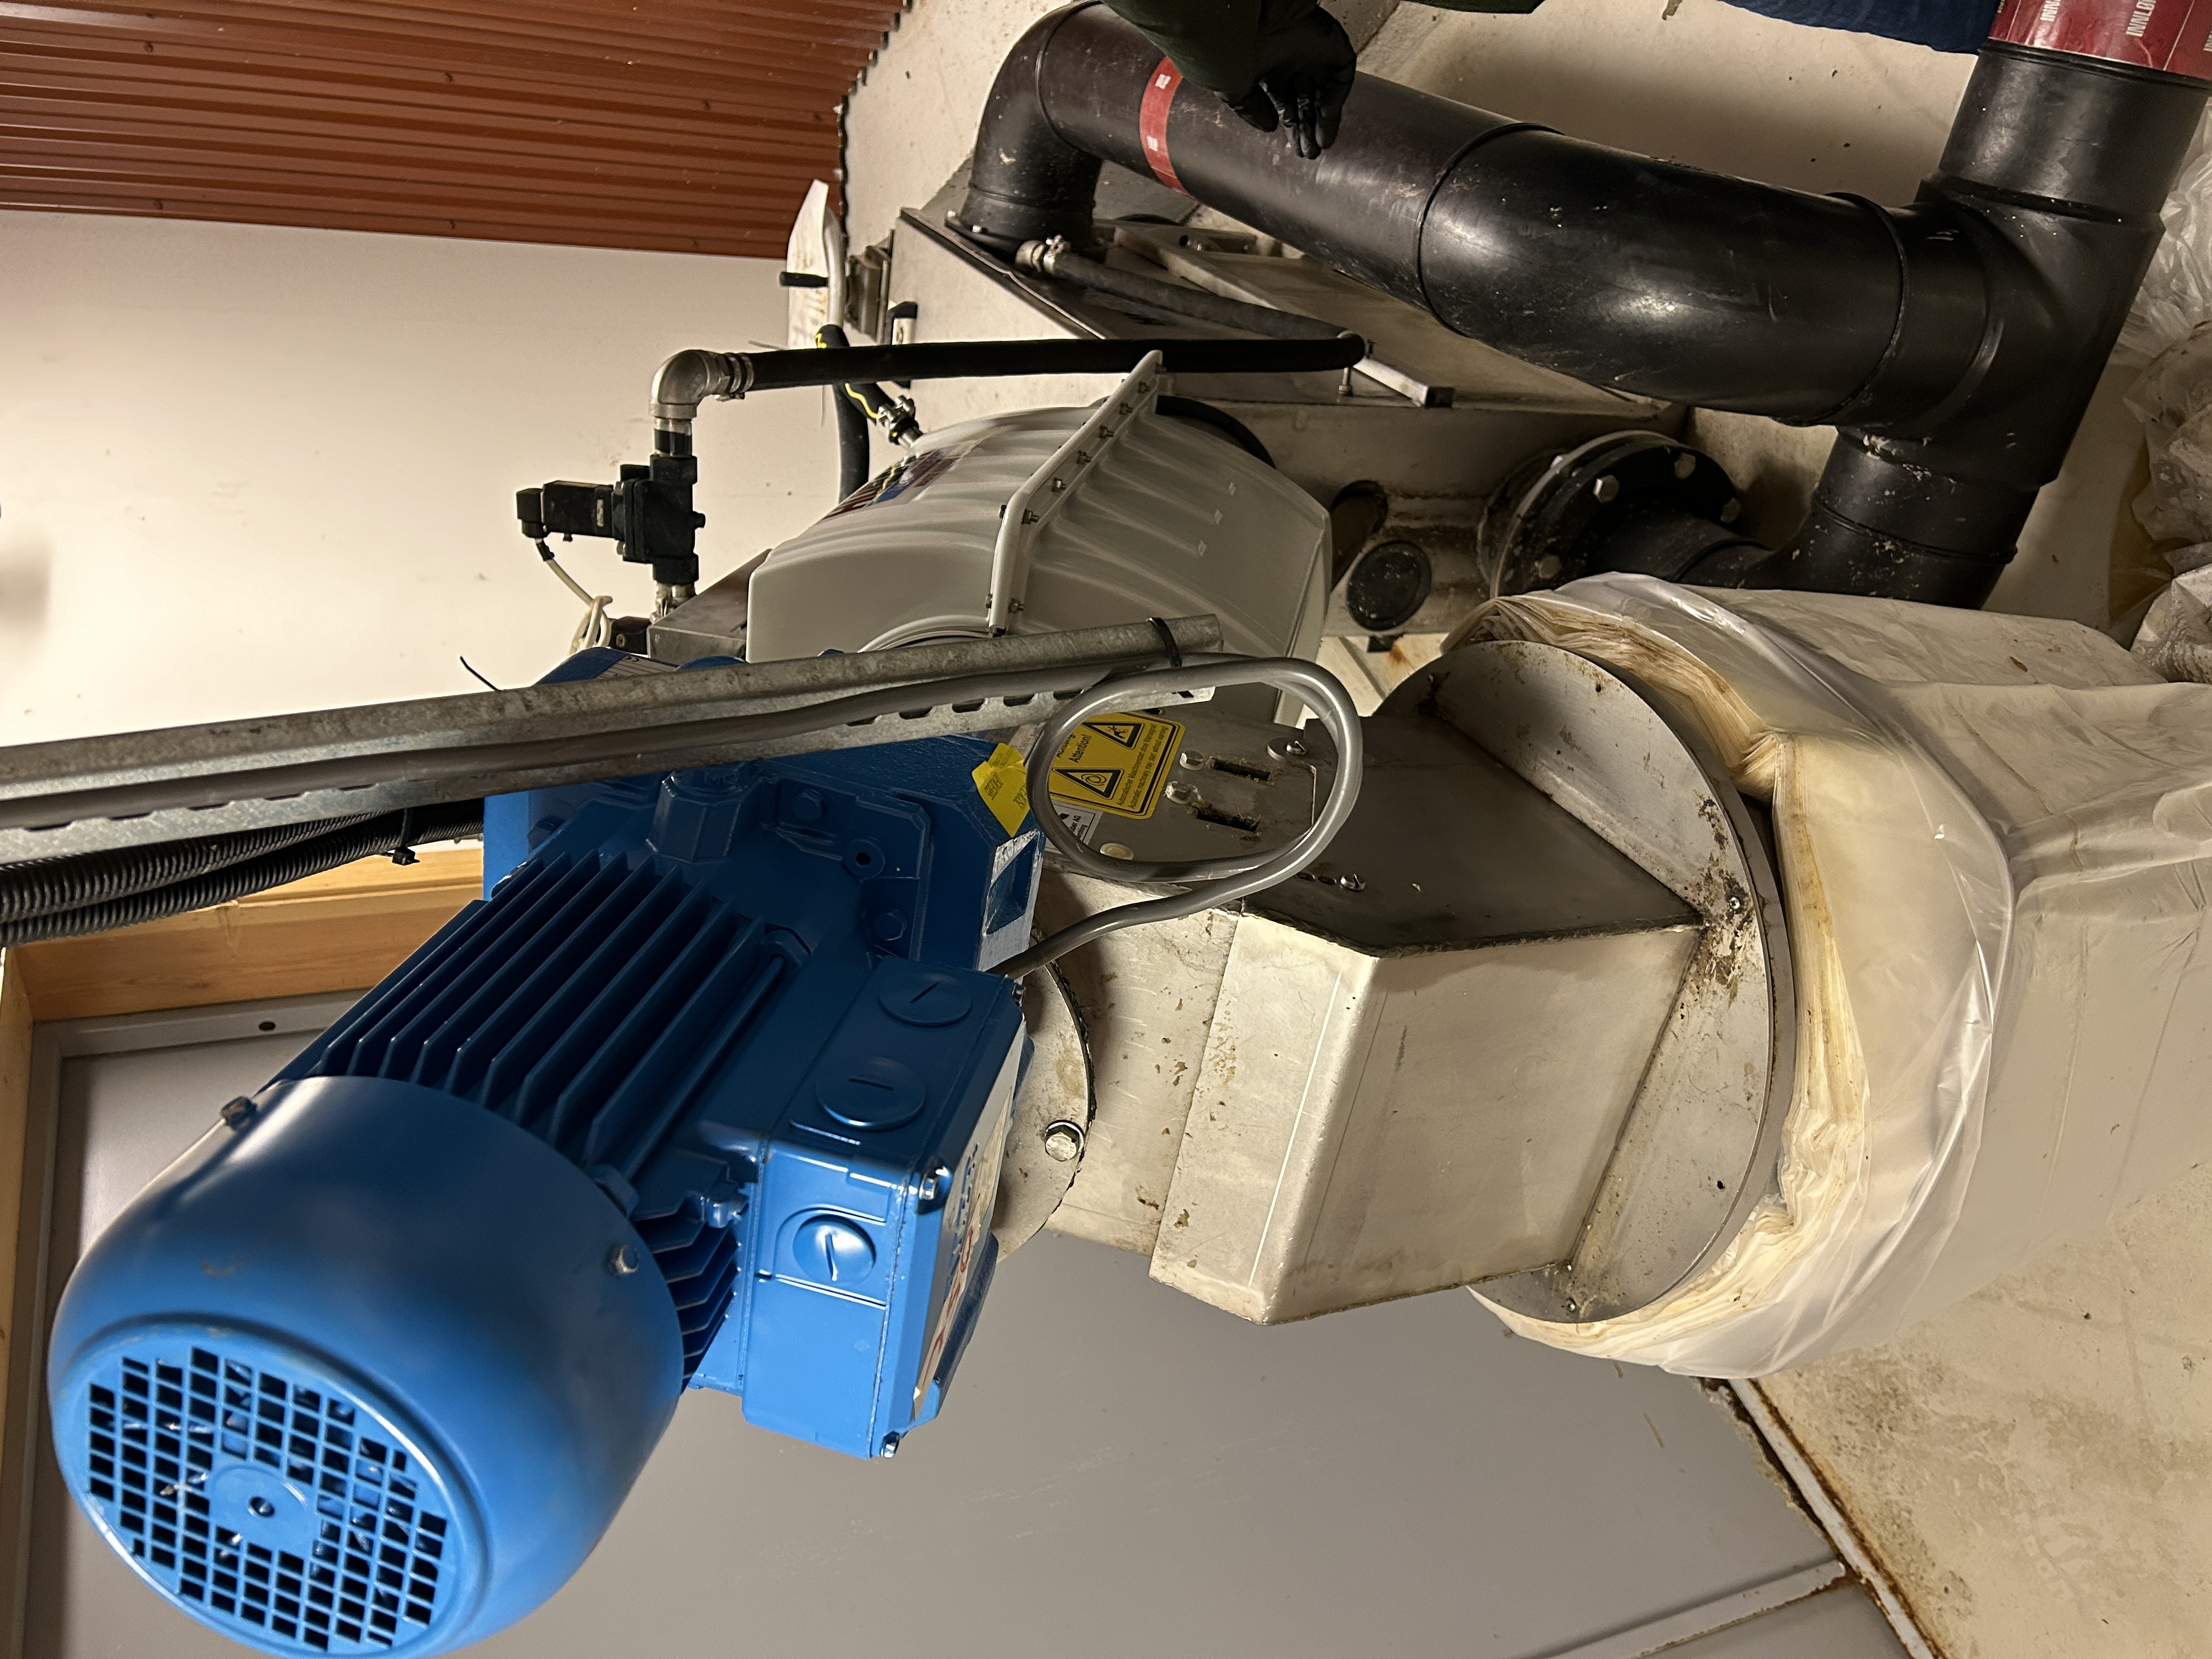
\includegraphics[angle=-90,width=1\textwidth]{Bilder/Huber.JPG}
        \caption{Motor og avfallshandtering}\label{fig:subfig1}
    \end{subfigure}
    \hfill
    \begin{subfigure}[b]{0.3\textwidth}
        \centering
        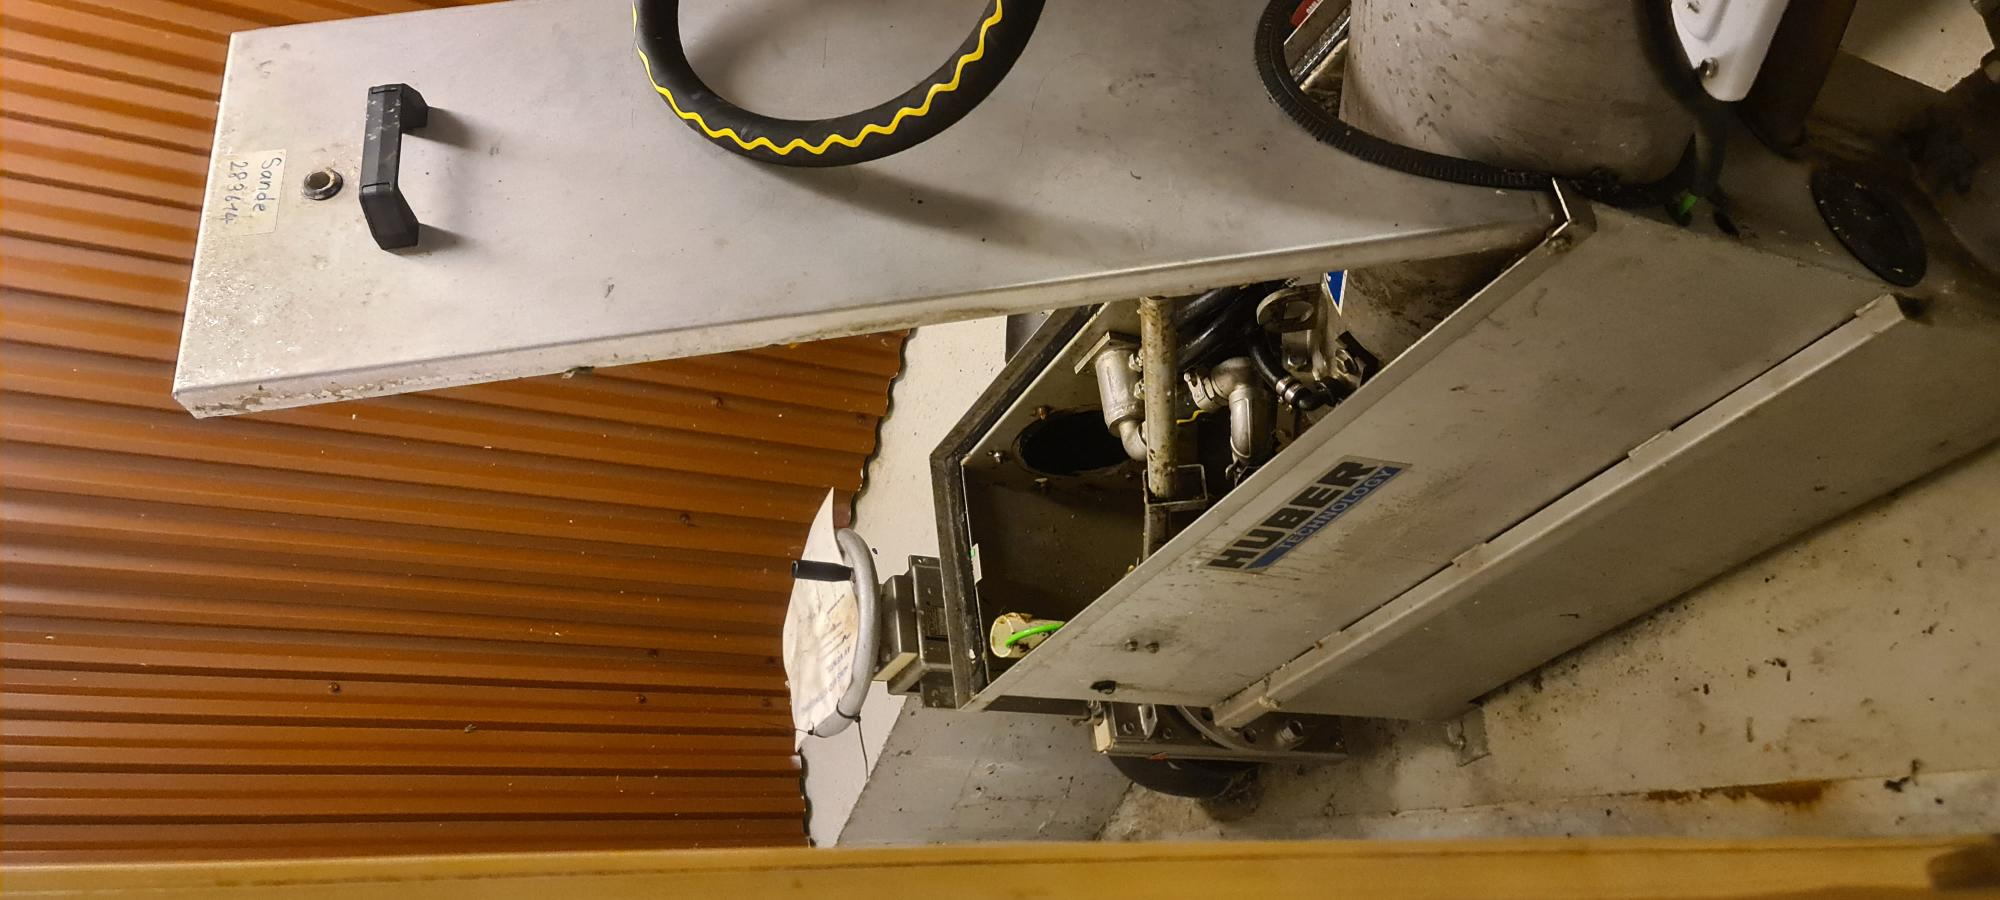
\includegraphics[angle=-90,width=0.6\textwidth]{Bilder/Huber2.JPG}
        \caption{Godts og skrue}\label{fig:subfig2}
    \end{subfigure}
    \caption{Bilete Huber grovrist}\label{fig:Illustrasjon-Diffuser}
\end{figure}

\newpage
\subsection{Mottakstank}
Frå grovrista renner vatnet med sjølvfall mot mottakstanken som ligger som lavaste punkt på anlegget.
Mottakstanken er 120 $m^3$ og er ein felles lagringsplass for vatnet før det går vidare mot reaktorane.
Mottakstanken har fire sensorar som heng ifrå taket.

\begin{itemize}
    \item Trykkgivar for nivå (PP00-LT01)
    \item Trykkgivar for overløp (PP00-LT02)
    \item Flottør-vippe lav (PP00-LS02)
    \item Flottør-vippe høg (PP00-LS01)  
\end{itemize}

Nivået i mottakstanken blir primært målt med trykkgivar LT01. For at vatnet skal pumpast vidare mot ein
reaktor i riktig sekvens må trykkgivar indikere at nivået er høgt nok. LS02 fungerar som backup.
I toppen av mottakstanken er det ei overløpskasse som drenerer mot resepient, her vil det
ved normale omstendigheter ikkje renne anna ein reinsavatn. Trykkgivar for overløp måler
dersom ureinsavatn renner i resepientrøyret.

%% Må endre på tegning fordi det eine navnet er feil. Ikkje reject frå sivbed.

\begin{figure}[htbp]
    \centering
    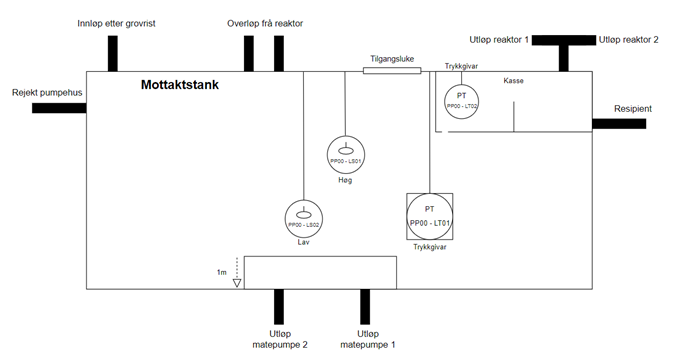
\includegraphics[width=1\textwidth]{Figurar/Mottakstank.png}
    \caption{Illustrasjon mottakstank}\label{fig:HMI}
\end{figure}

\begin{figure}[htbp]
    \centering
    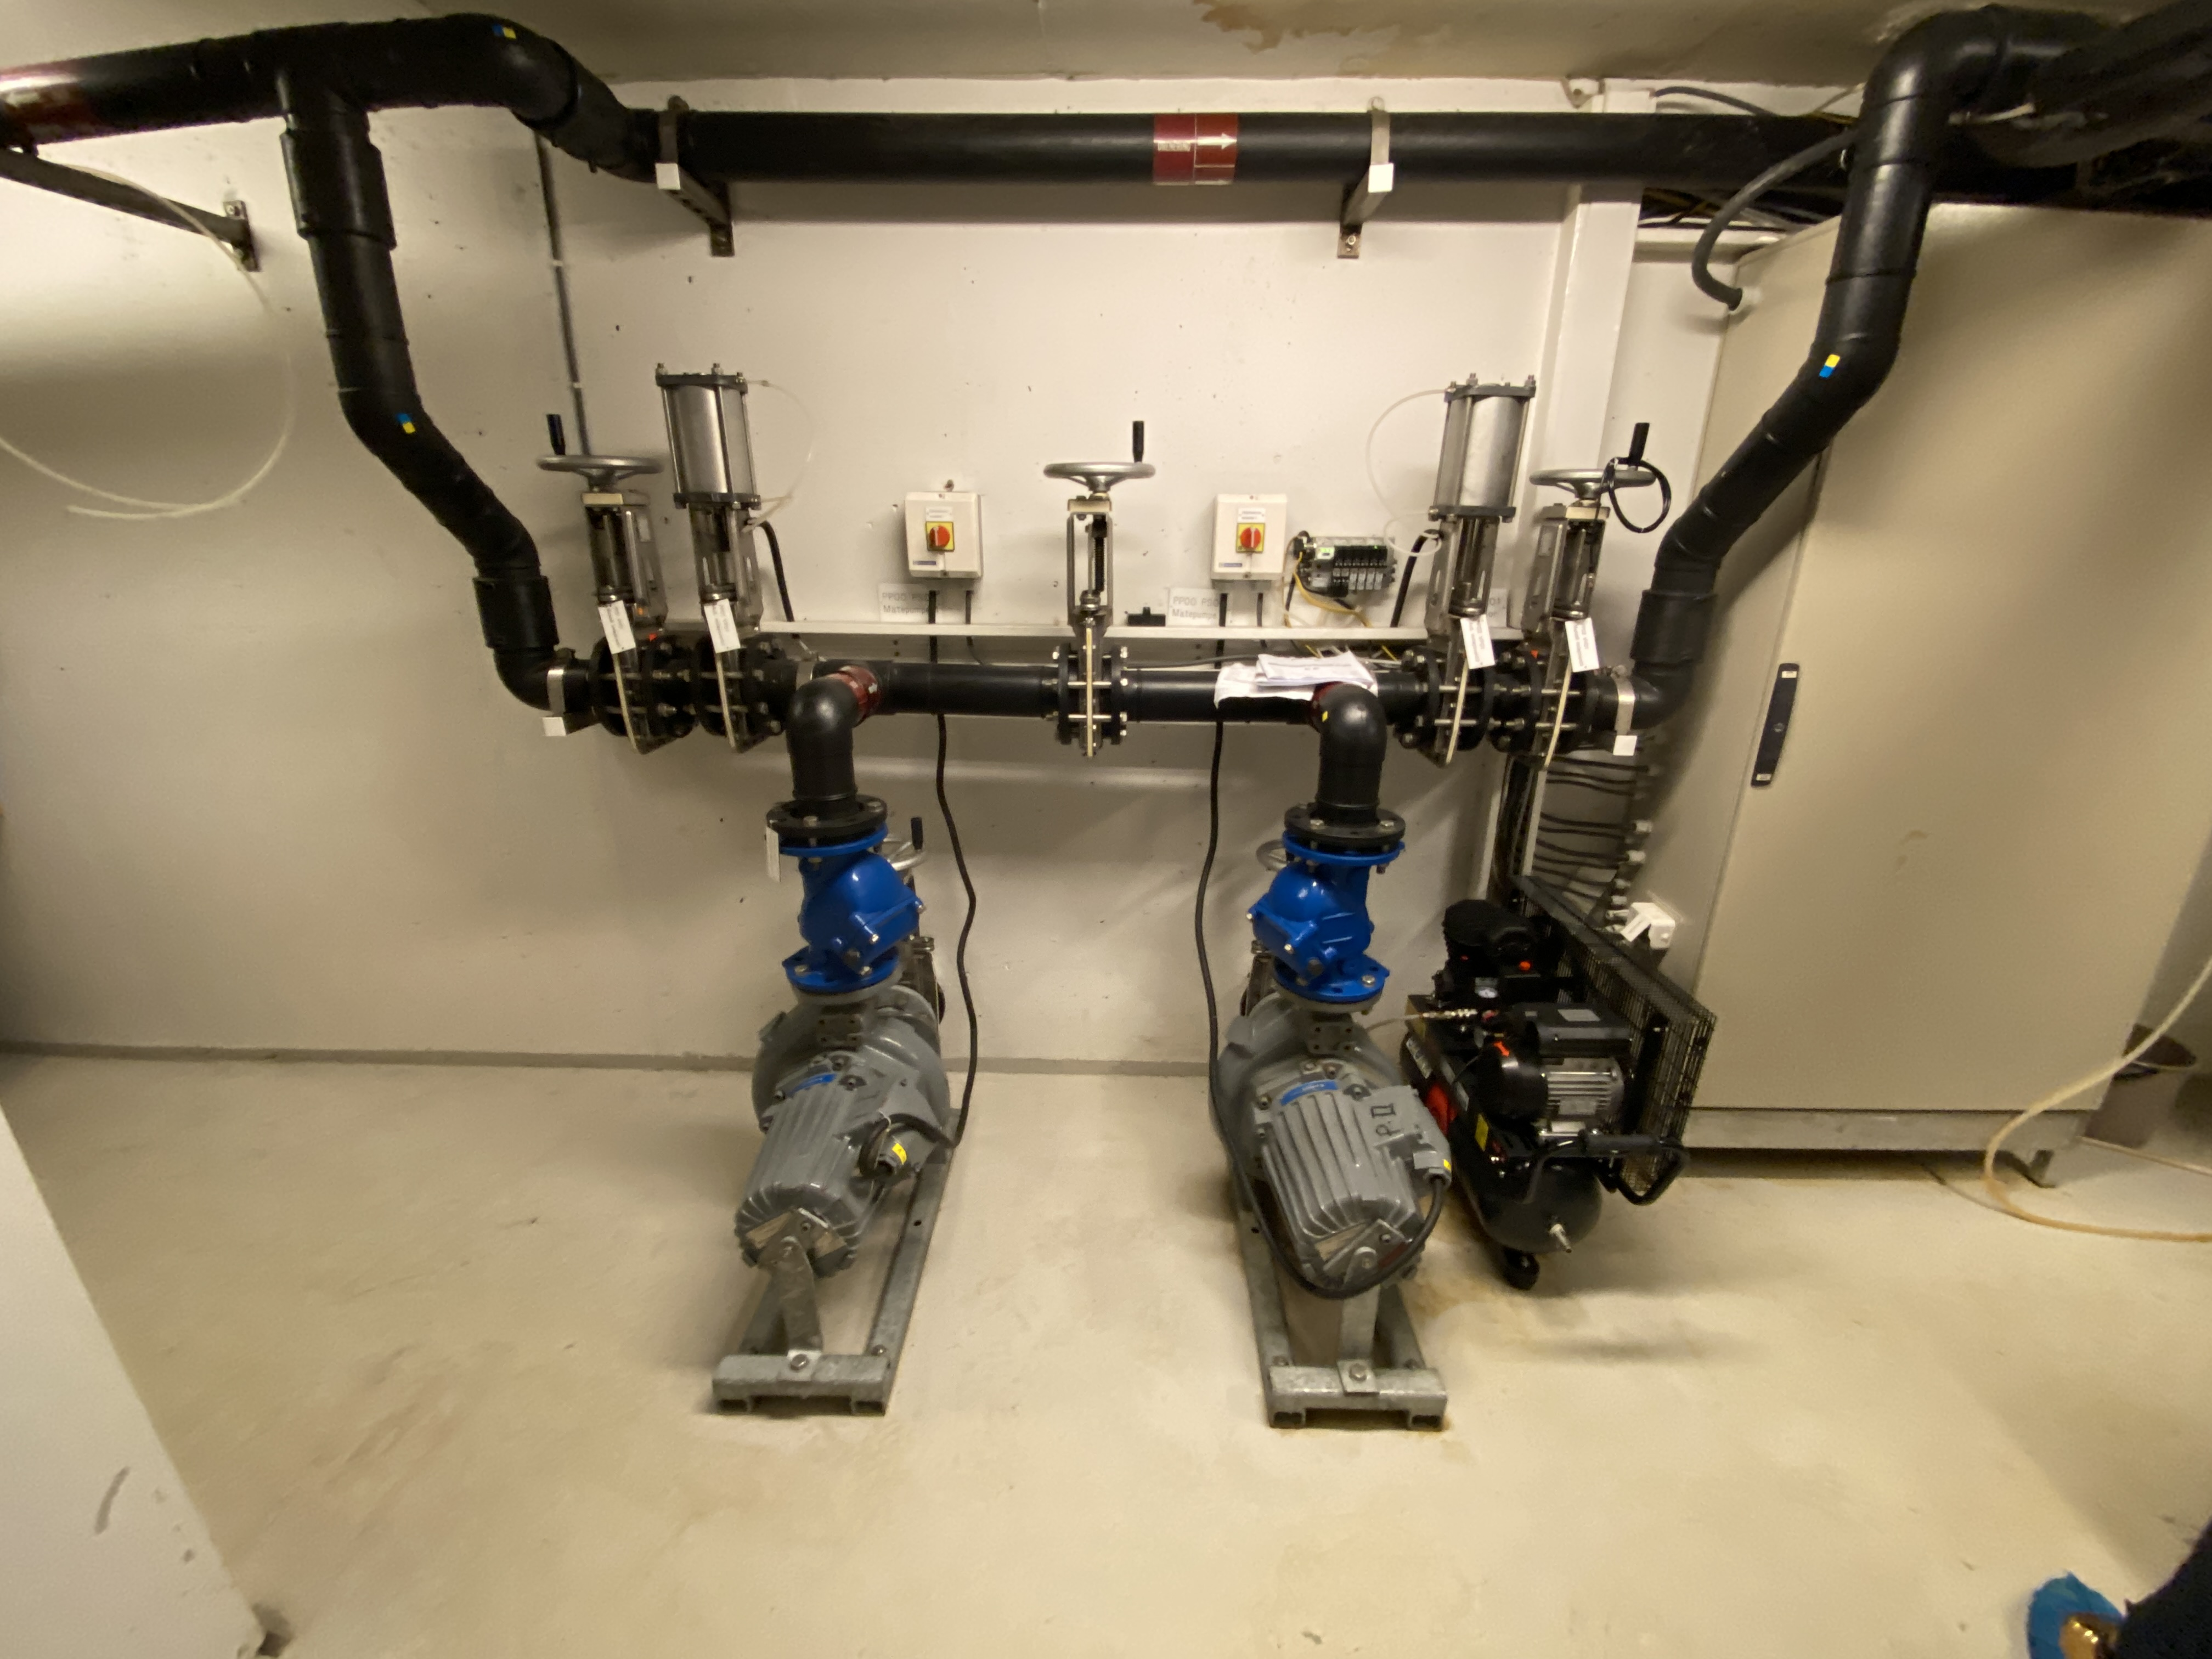
\includegraphics[width=1\textwidth]{Bilder/Bilde pumper.jpg}
    \caption{Matepumper Sande}\label{fig:HMI}
\end{figure}

\newpage
\subsection{Reaktor}

Frå mottakstanken blir vatnet pumpa opp mot ein reaktor dersom den er i riktig sekvens.
Vatnet blir pumpa opp ved hjelp av to matepumper som rullerer, og kvar pumpe kan
levere til kvar reaktor. 
Reaktorane står på bakkenivå og strekker seg opp mot taket på bygget.
Reaktorane er utstyrt med nivåmåling via trykk. Trykksensoren står ca to meter over bunn av reaktor.

I reaksjonssekvensen blir reaktorane periodisk lufta. Dette er for å lage aerobe og anokiske fasar
for mikroorganismane i reaktoraen som vidare gir betre reinsing.
For å for å best spreie oksygenet i den aerobe fasen
er det satt inn eit diffuser-oppsett i botn.
Diffurserane er laga av ein membran med små hull som dannar bobler når lufta kjem i 
kontakt med avlaupsvatnet.
Lufting av reaktoren gir også effektiv omrøring utan behov for ektra mekanisk inngrep.

\begin{figure}[htbp]
    \centering
    \begin{subfigure}[b]{0.3\textwidth}
        \centering
        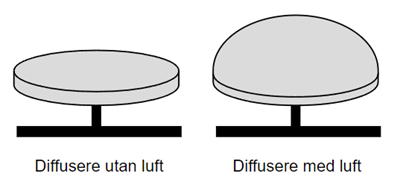
\includegraphics[width=1\textwidth]{Figurar/DiffusereMedOgUtanLuft.png}
        \caption{Illustrasjon diffuser}\label{fig:subfig1}
    \end{subfigure}
    \hfill
    \begin{subfigure}[b]{0.3\textwidth}
        \centering
        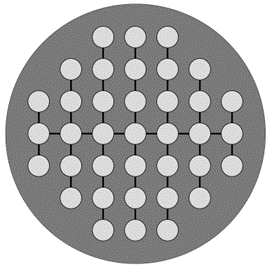
\includegraphics[width=1\textwidth]{Figurar/DiffuserFraTopp.png}
        \caption{Illustrasjon diffusere}\label{fig:subfig2}
    \end{subfigure}
    \caption{Illustrasjon oppsett av diffuser}\label{fig:Illustrasjon-Diffuser}
\end{figure}

På reiseanlegget er det ekstra krav for fjerning av fosfor. På grunn av desse ekstra krava
er det satt in eit tertiærreinse steg ved hjelp av simultanfelling.
Simultanfelling er ein fellesbetegnelse på kombinert biologisk og kjemisk reinsing.

I slutten på reaksjonsfasen tilsettest polyaluminium klorid, og kjemikaliet binder seg til
løyst fosfor og danner sedimenterbare partiklar. Desse sedimenterbare partiklane synker 
så i sedimenteringsfasen og utslippskravet på fosfor opprettholdast.

\begin{figure}[htbp]
    \centering
    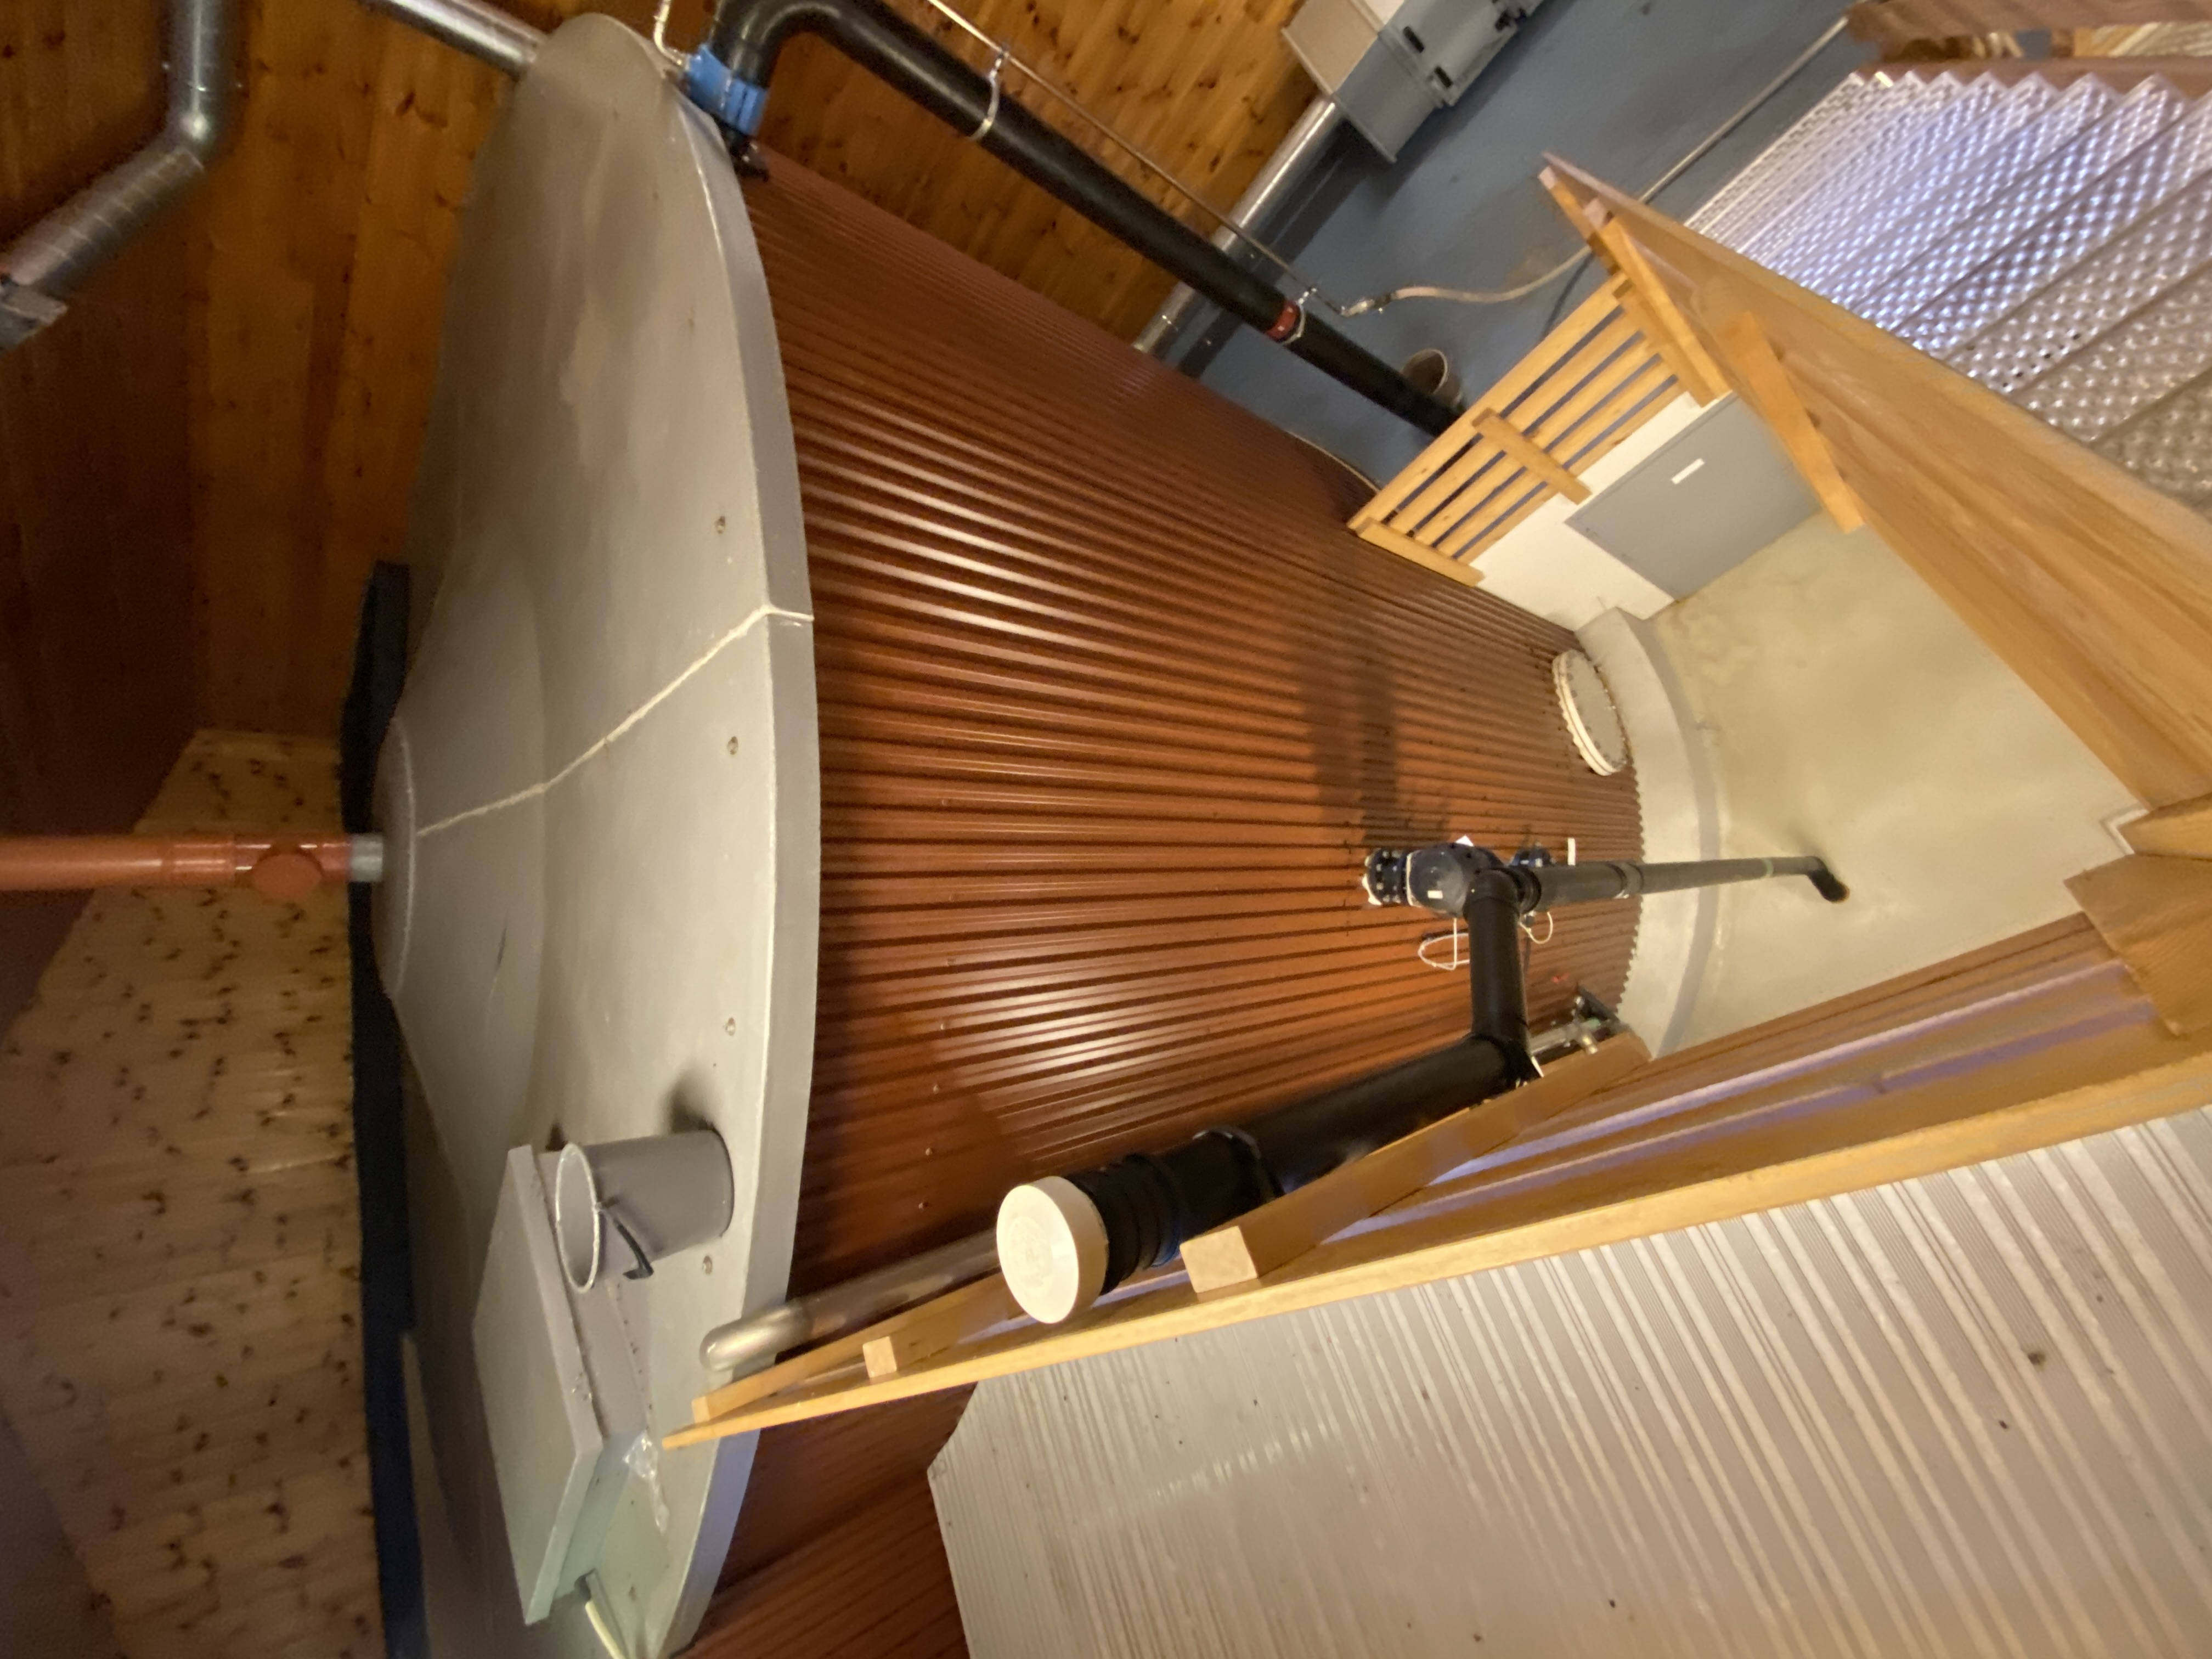
\includegraphics[angle=-90, width=1\textwidth]{Bilder/BildeReaktor.jpg}
    \caption{Reaktor Sande}\label{fig:reaktorsoner}
\end{figure}

\newpage

Reaktorane er delt opp i tre forskjellige soner. Desse sonene er med på å skille
dei forskjellige medium når reaktoren er ferdig med ein syklus.
Alle SBR-reaktorar har lagra aktivt slam i botn. Det er her alle mikroorganismane akkumulerast
og gir god biologisk reinsing. Denne sona blir kalla slamsona.\newline
Alt over uttaksventilen er definert som bruksvolumet til reaktoren og det
er dette volumet som blir fylt og behandla kvar innpumpingsekvens.

Mellom dei to sonene eksisterer der ei sikkerheitssone.
Denne sona er til for å ta hand om varierande sedimenteringseigenskapar
og overskuddslam. \newline

\begin{figure}[htbp]
    \centering
    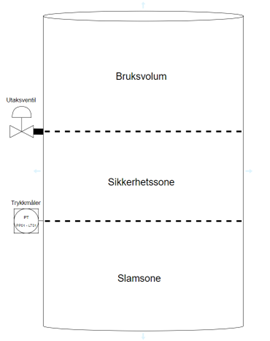
\includegraphics[width=0.5\textwidth]{Figurar/Reaktorsoner.png}
    \caption{Illustrasjon reaktorsoner}\label{fig:reaktorsoner}
\end{figure}

\subsection{P\&ID}

Det å setje seg inn i anleggets verkemåte skulle vise seg å være noko meir problematisk ein vi hadde forventa.
Hovudgrunnen til dette var at det ikkje fantest noko røyrgateskjema eller teknisk planteikning.
Vi ansåg det som naudvendig å etablere eit P\&ID diagram for å betre dokumentere og vise samanhengen til anlegget.

\begin{figure}[htbp]
    \centering
    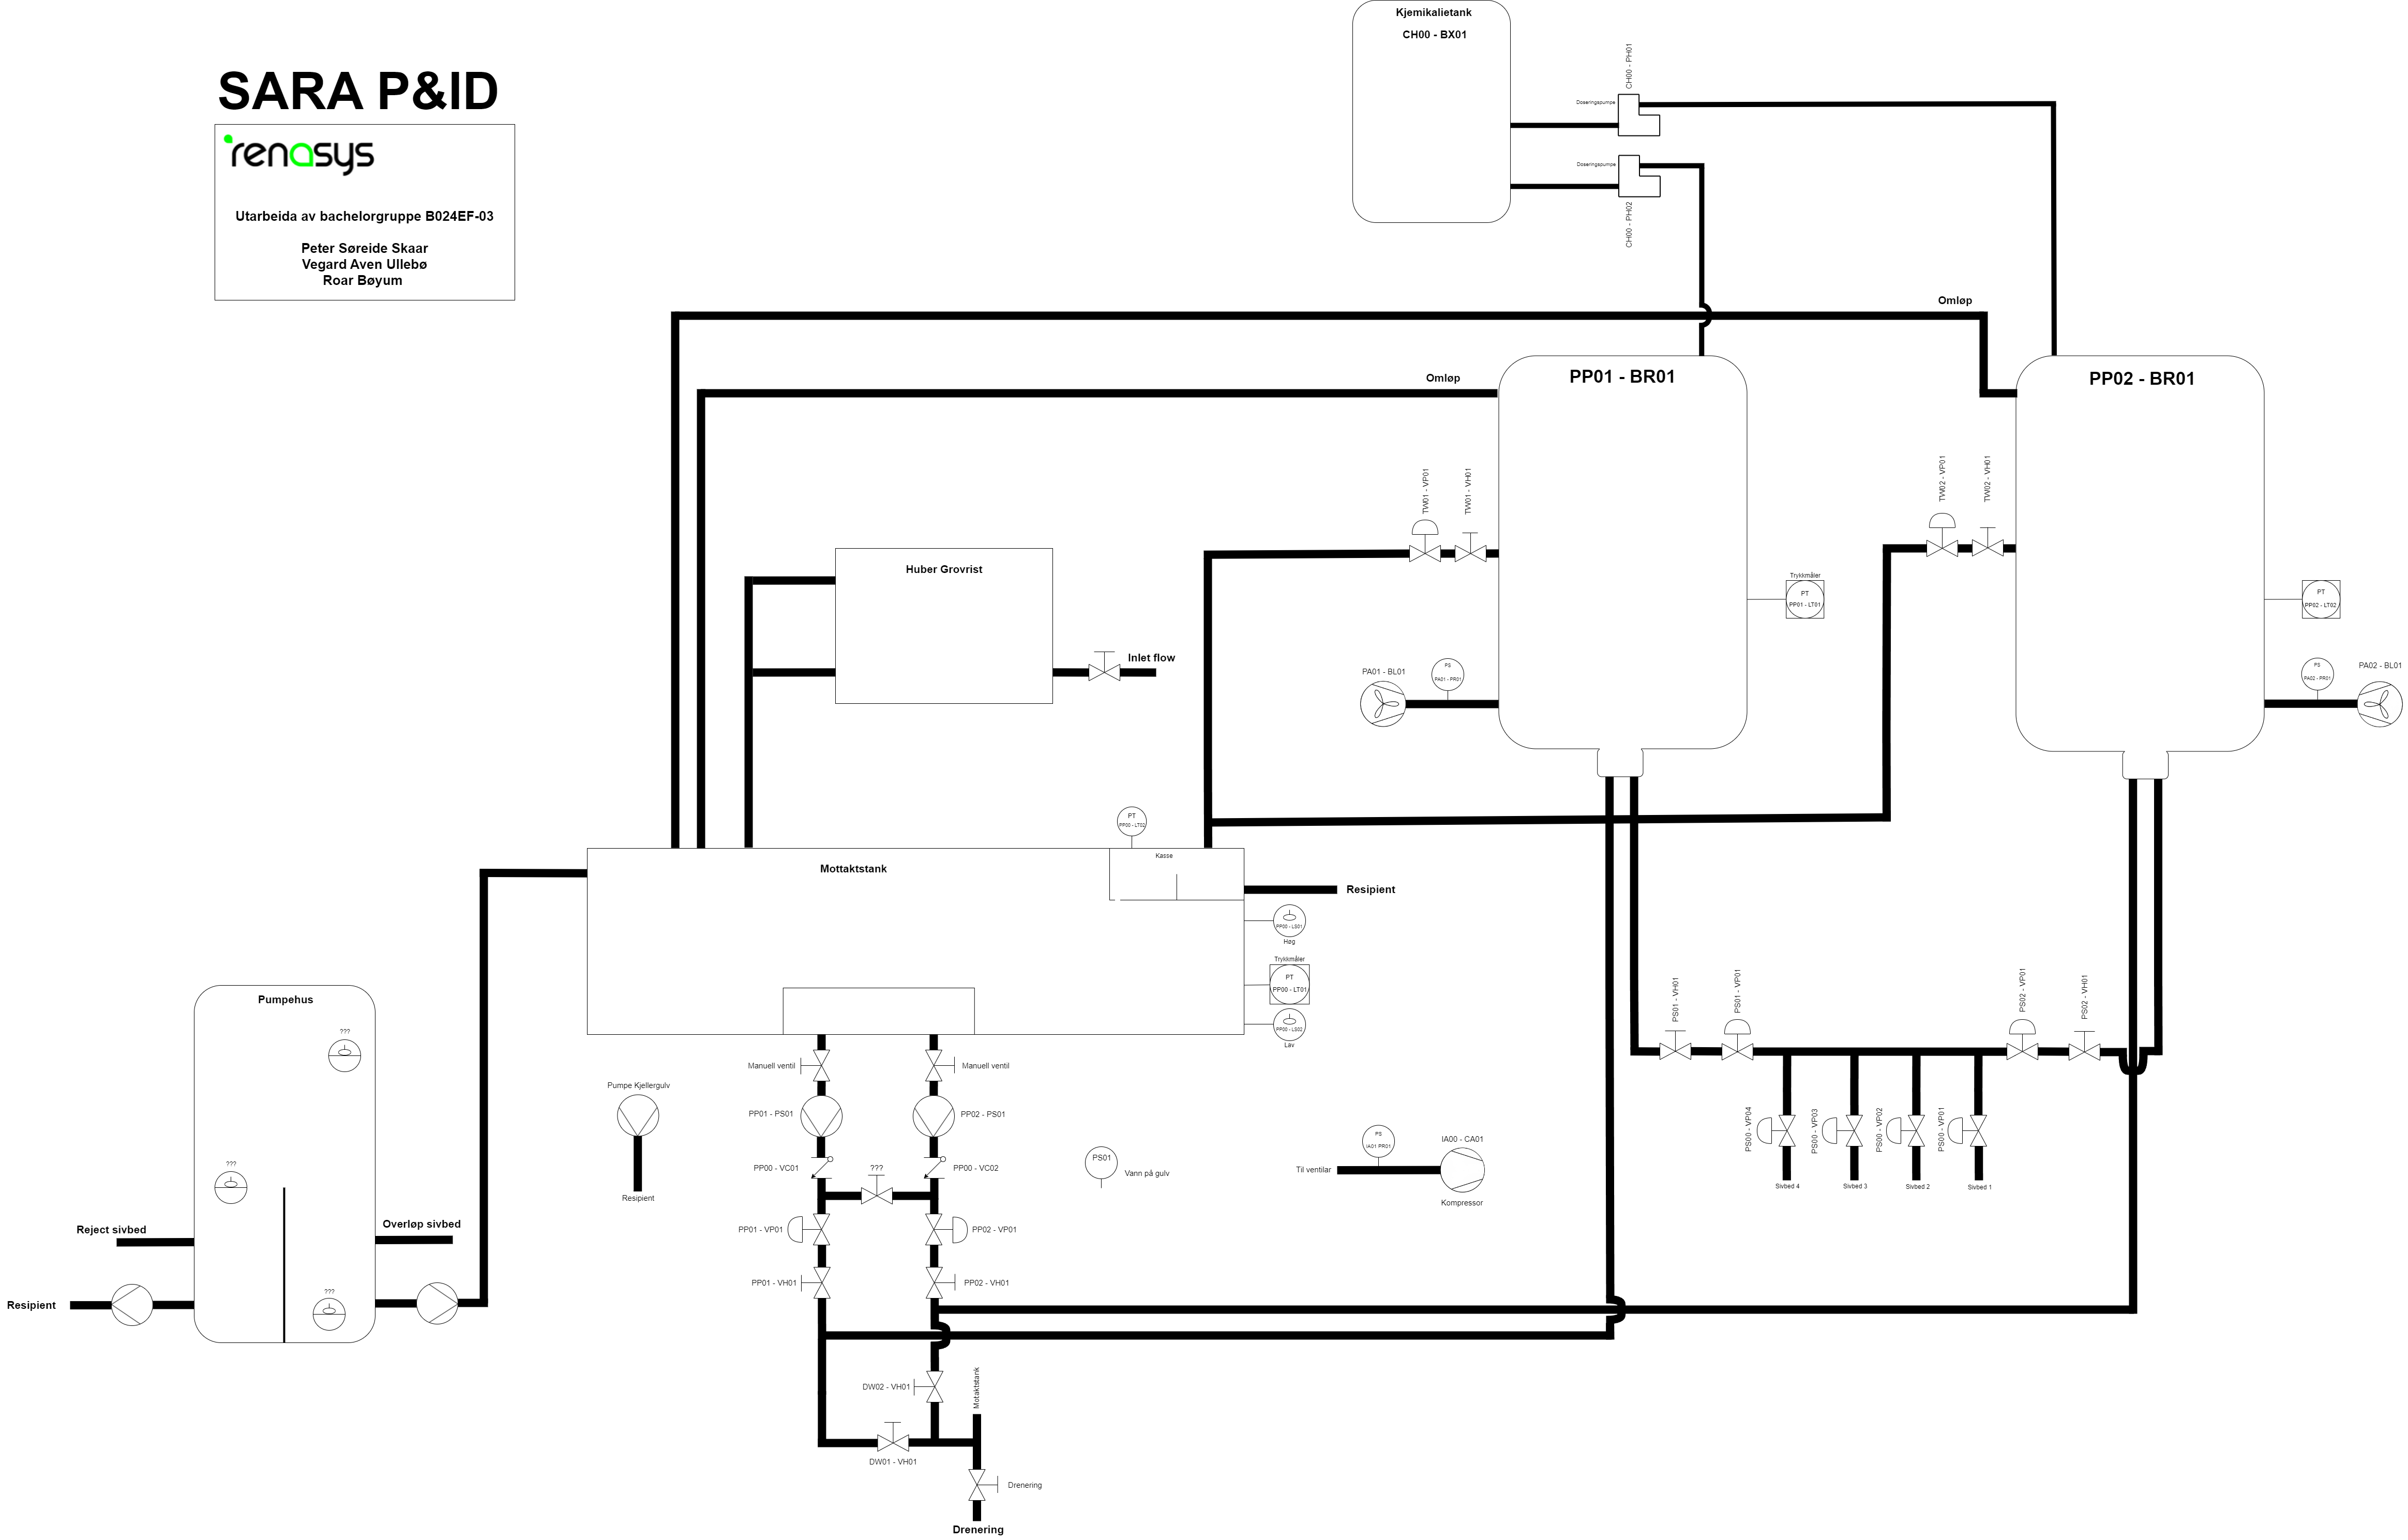
\includegraphics[angle=90,width=1\textwidth]{Figurar/P&ID.drawio.png}
    \caption{P\&ID}\label{fig:HMI}
\end{figure}